\documentclass{report}[a4paper]
% Decent underlines
\usepackage[normalem]{ulem}
% Hyperreferences
\usepackage{hyperref}
% Margins
\usepackage[top=35mm,bottom=35mm,left=25mm,right=25mm]{geometry}
% Graphics and images
\usepackage{graphicx} \graphicspath{{./images/}}
\usepackage{subcaption}
\usepackage{float}
% Encodings (to render letters with diacritics and special characters)
\usepackage[utf8]{inputenc}
% Language
\usepackage[english]{babel}
% Source code
\usepackage{listings}
\usepackage{xcolor}
\renewcommand{\lstlistingname}{File}
\lstset{
    frame=tb, % draw frame at top and bottom of the code
    tabsize=4, % tab space width
    numbers=left, % display line numbers on the left
	showstringspaces=false, % don't mark spaces in strings    
    commentstyle=\color{green}, % comment color
    keywordstyle=\color{blue}, % keyword color
    stringstyle=\color{red} % string color
}
\lstdefinelanguage{Maxima}{
	keywords={log,jacobian,determinant,subst},
	sensitive=true,
	comment=[n][\itshape]{/*}{*/}
}
% Tables with bold rows
\usepackage{tabularx}
\newcommand\setrow[1]{\gdef\rowmac{#1}#1\ignorespaces}
\newcommand\clearrow{\global\let\rowmac\relax}
\clearrow
\usepackage{multirow}
% Math stuff
\usepackage[mathscr]{euscript}
\usepackage{amsmath,amssymb}
\usepackage{mathtools}
\usepackage{enumitem}
\newcommand{\expnumber}[2]{{#1}\mathrm{e}{#2}} % scientific notation
% Definitions, theorems, remarks,...
\usepackage{amsthm}
\newtheorem{definition}{Definition}[section]
\newtheorem{theorem}{Theorem}[section]
\newtheorem{corollary}{Corollary}[theorem]
\newtheorem{lemma}[theorem]{Lemma}
\renewcommand\qedsymbol{$\blacksquare$}
\theoremstyle{remark}
\newtheorem*{remark}{Remark}
% Contents title
\addto\captionsenglish{\renewcommand*\contentsname{Table of contents}}
% Headers and footers
\usepackage{fancyhdr}
\pagestyle{fancyplain}
\fancyhf{}
\lhead{\fancyplain{}{Post office management database — Delivery II (BDAD 2019/20)}}
\rhead{\fancyplain{}{Group 605}}
\lfoot{\fancyplain{}{\leftmark}}
\rfoot{\thepage}
%
\newcommand{\email}[1]{
{\texttt{\href{mailto:#1}{#1}} }
}
% Metadata
\title{\Huge Post office management database \\ \Large Delivery II \\ \vspace*{4pt} \large BDAD 2019/20}
\author{
Group 605 \vspace{0.5em} \\
\begin{tabular}{r l}
	\email{up201806429@fe.up.pt} & Diogo Miguel Ferreira Rodrigues        \\
	\email{up201806613@fe.up.pt} & João António Cardoso Vieira e Basto de Sousa \\
	\email{up201806330@fe.up.pt} & Rafael Soares Ribeiro \\
\end{tabular}
}
\date{05/04/2020}
% Document
\begin{document}
\maketitle
\setcounter{tocdepth}{2}
\tableofcontents
\chapter{Introduction}
This preliminary report further details the project we proposed, improving on the previous report by including some minor corrections related to the UML Class Diagram and reflecting a better representation of the database required to solve the problem of managing a single post office, deliberately making little to no reference to the workings of a Postal Service given its complexity would greatly surpass recommendations. \par
A postal service is made up of post offices, where each post office has its own set of employees, vehicles and other attributes. The deliveries each have elements that influence its price as well as the ways they may be delivered and paid for, all of which will be explained more thoroughly through this report.\par
This version also includes the relational schema, functional dependencies, normal forms analysis and constraints aiming at maintaining data integrity.
\chapter{Conceptual model}
\section{Description}
\subsection{General classes}
\subsubsection{ZipCode}
Postal code (the designation of "ZIP code" is exclusive of the United States and some other countries, but since it conveys the same information with a shorter name we decided to adopt it), uniquely identified by the ISO 3166-1 alpha-2 country code (e.g., "PT") and code (e.g., "6120-111") and is characterized by the town (usually comes right after postal code; e.g., "PORTO") and by the postman in charge of distributing mail to postal addresses under that postal code (if there is one).
\subsubsection{Address}
An address is uniquely identified by an ID, and is characterized by its postal code (country and code), street name, street number (primary door number) and door number (fraction, floor number, etc.).
\subsubsection{PAddress}
A postal address extends an address by also mentioning a person name (addresser or addressee), thus being a subclass of Address. Besides mentioning an origin and destination, a delivery must also mention who the addresser and the addressee are, thus requiring a PAddress instead of an Address.\par
Since it only has an additional attribute relative to Address, this class was implemented by giving Address a personName attribute which can be NULL. If personName is NULL, it is a regular address, otherwise it is a PAddress.
\subsection{PostalService}
A postal service is a company that provides mail delivery services through its physical locations designated hereinafter post offices, one of them being the headquarters (implementation allows a NULL headquarters, since a PostOffice refers to a PostalService but a PostalService also refers to a specific PostOffice; since one of them has to be created first, we decided not to enforce a headquarters to be NOT NULL). It is uniquely identified by its VAT number, and is additionally characterized by the company name. \par
In this project, a PostalService serves the main purpose of storing the VAT and name of the entity that sells goods to clients, which avoids the need for thorough description of the workings of a PostalService that are not directly handled by a PostOffice.
\subsubsection{PostOffice}
Post offices are places of contact between the postal service and the clients, where services are provided and purchases take place. A PostOffice is associated with a single PostalService.\par
It is uniquely identified by an ID, and characterized also by its unique name, its address, a list of employees, and by the assigned vehicles. For this reason, it is directly connected to the classes PostalService, Address, Employee and Vehicle.
\subsubsection{Vehicle}
A vehicle is used to deliver mail and cannot be assigned to time-overlapping orders, given it can only fulfill an order at a time. It is uniquely identified by its license plate, and for each vehicle we know its capacity, that is, the maximum weight it can carry.
\subsubsection{Motorbike}
A motorbike is a vehicle which can be used to fulfill light orders, thus being a subclass of Vehicle.
\subsubsection{Van}
Like the motorbike, the van extends class Vehicle, but unlike the motorbike, it can be used to deliver general orders.
\subsection{Person}
For every person we know the VAT number (also serving as the unique person ID), name, address and phone number.
\subsubsection{Client}
A client is a person which may pay for a good or service via a Bill. It extends Person and does not have any additional attributes.
\subsubsection{Employee}
An employee is a person (thus a subclass of Person) that is employed by the company, which provides him/her with a salary. For every employee we know his/her base salary.
\subsubsection{Manager}
A manager is an employee who is responsible for monitoring a set of sales employees and postmen.
\subsubsection{ShopKeeper}
A shopKeeper is a sales Employee (thus extending the class Employee) who is responsible for processing sales and registering deliveries paid at the PostOffice and mail collected from postboxes.
\subsubsection{Postman}
A postman is an employee (therefore being a subclass of Employee) responsible for home-to-home mail distribution. A postman is assigned a group of postal codes.
\subsection{Delivery}
A delivery is requested by the client and registered by a shopKeeper. \par
Identifiable by its ID, each delivery keeps track of the time of registration, weight, and the postal addresses of the origin and destination (thus connecting this class to PAddress). A delivery’s price is determined not only by the type of service chosen (Economy, Express or Registered) but also by its category; it is classified as a Document if it weighs under 0.100kg, as Parcel if under 2.000kg or Overweight otherwise (up to 10.000kg).\par
Depending on the delivery, its payment can be done either by the purchase of a stamp (which is only valid should the delivery’s category be Document) and deposit at a postbox, or via a bill. A delivery paid via stamp has the fields numBill and seller as NULL.
\subsubsection{Order}
An order corresponds to a request of transporting a deliverable to its destination.\par
It is characterized by its identification number as well as by the postman assigned to its delivery, by the vehicle used for that end and by the scheduled time of departure from and arrival to the post office by the postman.\par
It can either be a General Order or a Light Order depending on the category (and therefore on the weight) of the deliverables: light orders can only be used for deliveries which have Documents as its category. A light order can be fulfilled by foot.
\subsubsection{Stamp}
A stamp is an alternative to paying for a Document using a bill. A stamped document can be deposited in a postbox. Given stamps are specialized according to the service that will be used in transporting the Document, Stamp is associated to the class Service.
\subsection{Bill}
A bill can be used to buy products at a PostOffice, as well as to pay for any kind of deliverable. A bill is uniquely identified by its bill number and seller's VAT (which is the company the client is paying for a delivery), and is described by the price (which is the sum of prices of the items of the delivery plus any other item bought at the PostOffice), issue time, issuing shopKeeper and the client that paid for it.
\subsubsection{CatalogItem}
A catalog item has a corresponding ID (similar to a bar-code), description and current price. The list of all catalog items make up the catalog of products the PostalService has for sale.
\subsubsection{BillItem}
A bill item represents a particular line in a Bill, meaning it identifies the kind of CatalogItem being bought, the price per unit at the moment it was bought, and the amount, for which a client paid a given sum. It is identifiable by the bill it belongs to (numBill and seller), plus the type of CatalogItem it refers to (since there cannot be two lines in the same bill referencing the same catalog product, and those two lines could rather be represented by a single line with the sum of the amounts).
\section{UML}
\begin{figure}[H] \centering
	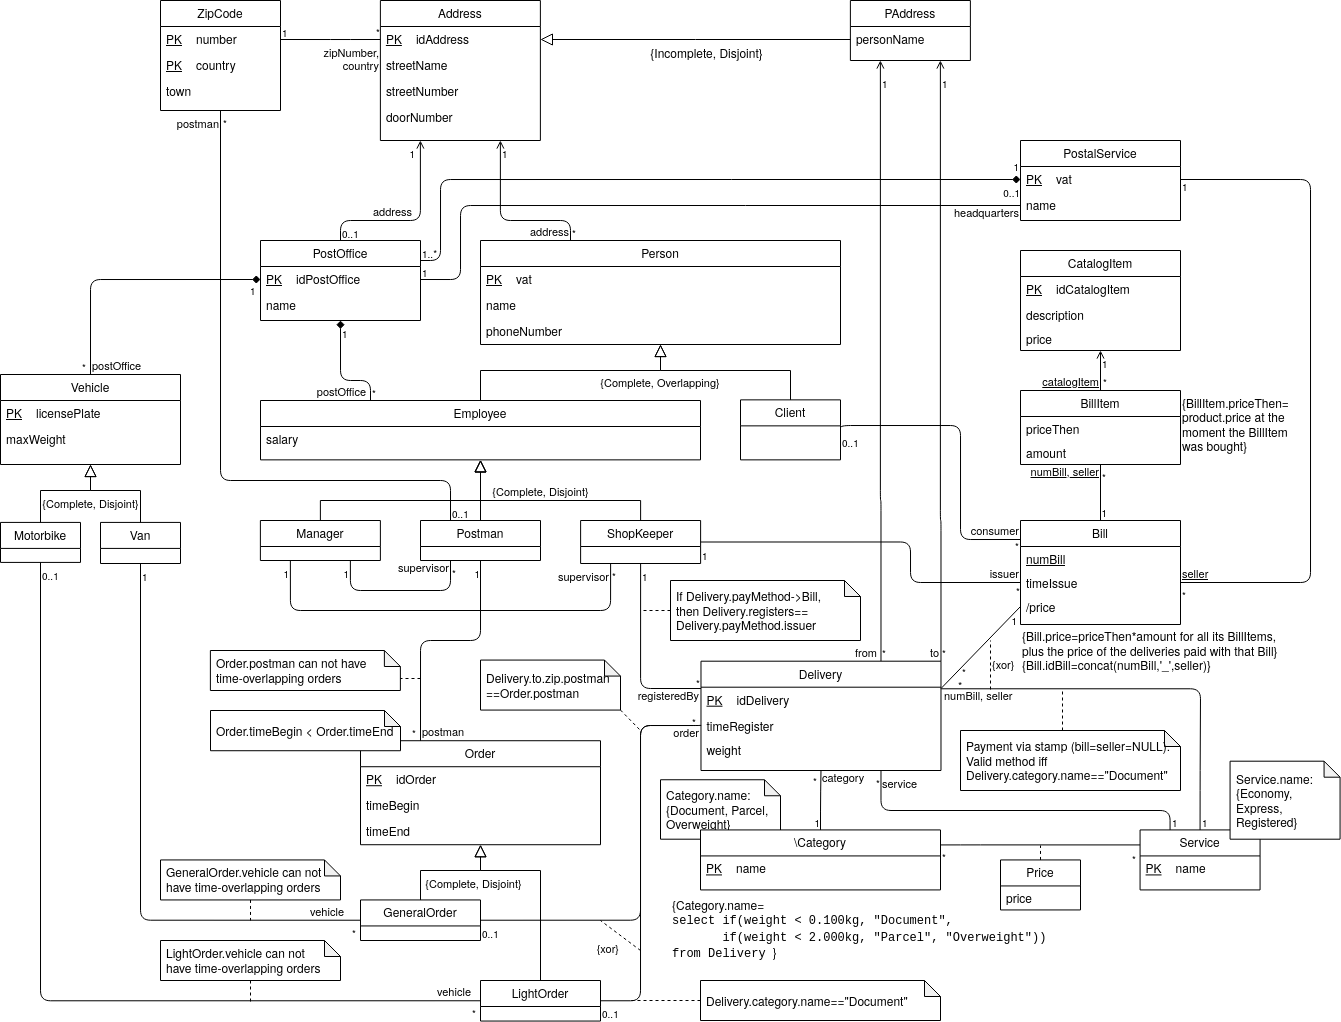
\includegraphics[angle=-90,scale=0.377]{uml2}
	\caption{Database UML}
\end{figure}
\chapter{Relational model}
\begin{center} \setlength{\tabcolsep}{1pt}
    \begin{tabular}{r p{144mm}}
        ZipCode         & (\uline{country}, \uline{number}, town, postman$\rightarrow$Postman)  \\
        Address         & (\uline{idAddress}, (zipNumber, country)$\rightarrow$ZipCode, streetName, streetNumber, doorNumber, personName) \\
        PostalService   & (\uline{vat}, name, headquarters$\rightarrow$PostOffice)              \\
        PostOffice      & (\uline{idPostOffice}, name, address$\rightarrow$Address, postalService$\rightarrow$PostalService) \\
        Vehicle         & (\uline{licensePlate}, postOffice$\rightarrow$PostOffice, maxWeight, type) \\
                        & $\text{type} \in \{\text{"motorbike"}, \text{"van"}\}$\\
        Person          & (\uline{vat}, name, address$\rightarrow$Address, phoneNumber)         \\
        Client          & (\uline{vat}$\rightarrow$Person)                                      \\
        Employee        & (\uline{vat}$\rightarrow$Person, postOffice$\rightarrow$PostOffice, salary) \\
        Manager         & (\uline{vat}$\rightarrow$Employee)                                    \\
        ShopKeeper      & (\uline{vat}$\rightarrow$Employee, supervisor$\rightarrow$Manager)    \\
        Postman         & (\uline{vat}$\rightarrow$Employee, supervisor$\rightarrow$Manager)    \\
        Delivery        & (\uline{idDelivery}, from$\rightarrow$PAddress, to$\rightarrow$PAddress, registeredBy$\rightarrow$ShopKeeper, order$\rightarrow$Order, timeRegister, weight, category, service, (numBill, seller)$\rightarrow$Bill) \\
        Order           & (\uline{idOrder}, timeBegin, timeEnd, type, vehicle$\rightarrow$Vehicle, postman$\rightarrow$Postman) \\
                        & $\text{type} \in \{\text{"generalOrder"}, \text{"lightOrder"}\}$\\
        Bill            & (\uline{numBill}, \uline{seller}$\rightarrow$PostalService, timeIssue, price, consumer$\rightarrow$Client, issuer$\rightarrow$ShopKeeper)                                   \\
        CatalogItem     & (\uline{idCatalogItem}, description, price)                           \\
        BillItem        & ((\uline{numBill}, \uline{seller})$\rightarrow$Bill, \uline{catalogItem}$\rightarrow$CatalogItem, priceThen, amount) \\
        Price           & (\uline{category}$\rightarrow$Category, \uline{service}$\rightarrow$Service, price)
    \end{tabular}
\end{center}
\chapter{Functional dependencies and normal forms}
\subsubsection{ZipCode}
\begin{alignat*}{2}
\{\text{country},\text{number}\} \rightarrow \{\text{town}, \text{postman}\}
\end{alignat*}
This relation is in the BCNF, given that, in all nontrivial functional dependencies of the form $\overline{\text{A}} \rightarrow \overline{\text{B}}$ in this relation, $\overline{\text{A}}$ is a superkey. Since BCNF is a subset of 3NF, this relation is also in the 3NF.
\subsubsection{Address}
\begin{alignat*}{2}
    \{\text{idAddress}\} \rightarrow \{\text{zipNumber}, \text{country}, \text{streetName}, \text{streetNumber}, \text{doorNumber}, \text{personName}\}
\end{alignat*}
This relation is in the BCNF, given that, in all nontrivial functional dependencies of the form $\overline{\text{A}} \rightarrow \overline{\text{B}}$ in this relation, $\overline{\text{A}}$ is a superkey. Since BCNF is a subset of 3NF, this relation is also in the 3NF.
\subsubsection{PostalService}
\begin{alignat*}{2}
    \{\text{vat}\} \rightarrow \{\text{name},\text{headquarters}\}
\end{alignat*}
This relation is in the BCNF, given that, in all nontrivial functional dependencies of the form $\overline{\text{A}} \rightarrow \overline{\text{B}}$ in this relation, $\overline{\text{A}}$ is a superkey. Since BCNF is a subset of 3NF, this relation is also in the 3NF.
\subsubsection{PostOffice}
\begin{alignat*}{2}
    \{\text{idPostOffice}\} &\rightarrow \{\text{name},\text{address},\text{postalService}\} \\
    \{\text{name}\} &\rightarrow \{\text{idPostOffice}\} \\
\end{alignat*}
This relation is in the BCNF, given that, in all nontrivial functional dependencies of the form $\overline{\text{A}} \rightarrow \overline{\text{B}}$ in this relation, $\overline{\text{A}}$ is a superkey (including $\{\text{name}\}$, given that $\{\text{name}\}^+ = \{\text{name}, \text{idPostOffice}\}^+ = \{\text{name}, \text{idPostOffice}, \text{address}, \text{postalService}\}$). Since BCNF is a subset of 3NF, this relation is also in the 3NF.
\subsubsection{Vehicle}
\begin{alignat*}{2}
    \{\text{licensePlate}\} \rightarrow \{\text{postOffice},\text{maxWeight},\text{type}\}
\end{alignat*}
This relation is in the BCNF, given that, in all nontrivial functional dependencies of the form $\overline{\text{A}} \rightarrow \overline{\text{B}}$ in this relation, $\overline{\text{A}}$ is a superkey. Since BCNF is a subset of 3NF, this relation is also in the 3NF.
\subsubsection{Person}
\begin{alignat*}{2}
    \{\text{vat}\} \rightarrow \{\text{name},\text{address},\text{phoneNumber}\}
\end{alignat*}
This relation is in the BCNF, given that, in all nontrivial functional dependencies of the form $\overline{\text{A}} \rightarrow \overline{\text{B}}$ in this relation, $\overline{\text{A}}$ is a superkey. Since BCNF is a subset of 3NF, this relation is also in the 3NF.
\subsubsection{Client}
\begin{alignat*}{2}
    \{\text{vat}\} \rightarrow \{\text{name},\text{address},\text{phoneNumber}\}
\end{alignat*}
This relation is in the BCNF, given that, in all nontrivial functional dependencies of the form $\overline{\text{A}} \rightarrow \overline{\text{B}}$ in this relation, $\overline{\text{A}}$ is a superkey. Since BCNF is a subset of 3NF, this relation is also in the 3NF.
\subsubsection{Employee}
\begin{alignat*}{2}
    \{\text{vat}\} \rightarrow \{\text{name},\text{address},\text{phoneNumber},\text{postOffice},\text{salary}\}
\end{alignat*}
This relation is in the BCNF, given that, in all nontrivial functional dependencies of the form $\overline{\text{A}} \rightarrow \overline{\text{B}}$ in this relation, $\overline{\text{A}}$ is a superkey. Since BCNF is a subset of 3NF, this relation is also in the 3NF.
\subsubsection{Manager}
\begin{alignat*}{2}
    \{\text{vat}\} \rightarrow \{\text{name},\text{address},\text{phoneNumber},\text{postOffice},\text{salary}\}
\end{alignat*}
This relation is in the BCNF, given that, in all nontrivial functional dependencies of the form $\overline{\text{A}} \rightarrow \overline{\text{B}}$ in this relation, $\overline{\text{A}}$ is a superkey. Since BCNF is a subset of 3NF, this relation is also in the 3NF.
\subsubsection{ShopKeeper}
\begin{alignat*}{2}
    \{\text{vat}\} \rightarrow \{\text{name},\text{address},\text{phoneNumber},\text{postOffice},\text{salary}, \text{supervisor}\}
\end{alignat*}
This relation is in the BCNF, given that, in all nontrivial functional dependencies of the form $\overline{\text{A}} \rightarrow \overline{\text{B}}$ in this relation, $\overline{\text{A}}$ is a superkey. Since BCNF is a subset of 3NF, this relation is also in the 3NF.
\subsubsection{Postman}
\begin{alignat*}{2}
    \{\text{vat}\} \rightarrow \{\text{name},\text{address},\text{phoneNumber},\text{postOffice},\text{salary}, \text{supervisor}\}
\end{alignat*}
This relation is in the BCNF, given that, in all nontrivial functional dependencies of the form $\overline{\text{A}} \rightarrow \overline{\text{B}}$ in this relation, $\overline{\text{A}}$ is a superkey. Since BCNF is a subset of 3NF, this relation is also in the 3NF.
\subsubsection{Delivery}
\begin{alignat*}{2}
    \{\text{idDelivery}\} &\rightarrow \{\text{from},\text{to},\text{registeredBy},\text{order},\text{timeRegister},\text{weight},\text{service},\text{numBill},\text{seller}\} \\
    \{\text{weight}\} &\rightarrow \{\text{category}\}
\end{alignat*}
This relation is in the 1NF, given the domain of each attribute contains only atomic values, and that the value of each attribute contains only a single value from that domain (in short, no attribute is a list/set, but rather an atomic value).\par
It is also in the 2NF, given $\{\text{idDelivery}\}$ is a candidate key (we thus ignore the first dependency), added to the fact that, although category is non-prime, $\{\text{weight}\}$ is not a proper subset of a candidate key. \par
It is not however in the 3NF, given the second functional dependency is a 3NF-violation since $\{\text{weight}\}$ is not a superkey nor is category a prime attribute. Since BCNF is a subset of 3NF, then the second functional dependency is also a BCNF-violation.\par
This violation takes place because this attribute's value is directly calculated from weight, which is but a consequence of the method presented in this course for transforming the UML into a list of relations, which suggests translating derivable UML attributes into regular relational attributes associated to their respective functional dependencies. \par
Had we considered this attribute to be calculated on-the-fly as a temporary variable, this violation would not take place. This is in fact the approach we will take to compress this particular table, thus meaning the actual database will not include the aforementioned violation.
\subsubsection{Order}
\begin{alignat*}{2}
    \{\text{idOrder}\} \rightarrow \{\text{timeBegin},\text{timeEnd},\text{type},\text{vehicle},\text{postman}\}
\end{alignat*}
This relation is in the BCNF, given that, in all nontrivial functional dependencies of the form $\overline{\text{A}} \rightarrow \overline{\text{B}}$ in this relation, $\overline{\text{A}}$ is a superkey. Since BCNF is a subset of 3NF, this relation is also in the 3NF.
\subsubsection{Bill}
\begin{alignat*}{2}
    \{\text{numBill},\text{seller}\} \rightarrow \{\text{timeIssue},\text{price},\text{consumer},\text{issuer}\}
\end{alignat*}
This relation is in the BCNF, given that, in all nontrivial functional dependencies of the form $\overline{\text{A}} \rightarrow \overline{\text{B}}$ in this relation, $\overline{\text{A}}$ is a superkey. Since BCNF is a subset of 3NF, this relation is also in the 3NF.
\subsubsection{CatalogItem}
\begin{alignat*}{2}
    \{\text{idCatalogItem}\} \rightarrow \{\text{description},\text{price}\}
\end{alignat*}
This relation is in the BCNF, given that, in all nontrivial functional dependencies of the form $\overline{\text{A}} \rightarrow \overline{\text{B}}$ in this relation, $\overline{\text{A}}$ is a superkey. Since BCNF is a subset of 3NF, this relation is also in the 3NF.
\subsubsection{BillItem}
\begin{alignat*}{2}
    \{\text{numBill},\text{seller},\text{catalogItem}\} \rightarrow \{\text{priceThen},\text{amount}\}
\end{alignat*}
This relation is in the BCNF, given that, in all nontrivial functional dependencies of the form $\overline{\text{A}} \rightarrow \overline{\text{B}}$ in this relation, $\overline{\text{A}}$ is a superkey. Since BCNF is a subset of 3NF, this relation is also in the 3NF.
\subsubsection{Price}
\begin{alignat*}{2}
    \{\text{category},\text{service}\} \rightarrow \{\text{price}\}
\end{alignat*}
This relation is in the BCNF, given that, in all nontrivial functional dependencies of the form $\overline{\text{A}} \rightarrow \overline{\text{B}}$ in this relation, $\overline{\text{A}}$ is a superkey. Since BCNF is a subset of 3NF, this relation is also in the 3NF.

\chapter{Restrictions}
\subsubsection{ZipCode}
\begin{itemize}
    \item Each ZipCode must have an associated town. \\ town VARCHAR(63) NOT NULL
    \item Each ZipCode may refer to a postman responsible for delivering mail in that area. \\ postman CHAR(15) REFERENCES Postman(vat)
    \item Each ZipCode is identifiable by the country and number. \\ PRIMARY KEY (country, code)
\end{itemize}
\subsubsection{Address}
\begin{itemize}
    \item Each address is identified by its id. \\ id INT PRIMARY KEY
    \item An address must have a zipCode associated with it. \\ zipCode CHAR(12) NOT NULL
    \item An address must have a country associated with it. \\ country CHAR(2) NOT NULL
    \item An address must have a street name associated with it. \\ streetName NOT NULL
    \item An address must have a street number associated with it. \\ streetNumber NOT NULL
    \item An address's zipCode and country reference its ZipCode. \\ FOREIGN KEY (zipCode, country) REFERENCES ZipCode(code, country)
\end{itemize}
\subsubsection{PostalService}
\begin{itemize}
    \item A PostalService is recognized by its VAT number. \\ vat CHAR(15) PRIMARY KEY
    \item Each PostalService must have a name. \\ name VARCHAR(255) NOT NULL
    \item Each PostalService has a headquarters, a special PostOffice, referenced by its id. \\ hq INT REFERENCES PostOffice(id)
\end{itemize}
\subsubsection{PostOffice}
\begin{itemize}
    \item A PostOffice is identifiable by its id. \\ id INT PRIMARY KEY
    \item PostOffice must have a name and there cannot be two PostOffices with the same name. \\ name VARCHAR(255) NOT NULL UNIQUE
    \item A PostOffice must have a non-null address. \\ address INT NOT NULL REFERENCES Address(id)
    \item A PostOffice belongs to a certain PostalService. \\ postalService CHAR(15) NOT NULL REFERENCES PostalService(vat)
\end{itemize}
\subsubsection{Vehicle}
\begin{itemize}
    \item A vehicle is recognized by its licensePlate. \\ plate CHAR(15) PRIMARY KEY
    \item A vehicle belongs to a specific PostOffice. \\ postOffice INT NOT NULL REFERENCES PostOffice(id)
    \item The maximum weight a vehicle can transport must be a positive value. \\ maxWeight FLOAT CHECK (maxWeight $>$ 0)
    \item There are only 2 types of vehicles: motorbike and van. \\ type CHAR(15) CHECK (type in ('motorbike', 'van'))
\end{itemize}
\subsubsection{Person}
\begin{itemize}
    \item A Person is identifiable by its VAT number. \\ vat CHAR(15) PRIMARY KEY
    \item A Person must have a name. \\ name VARCHAR(255) NOT NULL
    \item A Person must have an address. \\ address INT NOT NULL REFERENCES Address(id)
\end{itemize}
\subsubsection{Client}
\begin{itemize}
    \item As in the case of Person, a Client is identified by its VAT number. \\ vat CHAR(15) PRIMARY KEY REFERENCES Person
\end{itemize}
\subsubsection{Employee}
\begin{itemize}
    \item As in the case of Person, an Employee is identified by its VAT number. \\ vat CHAR(15) PRIMARY KEY REFERENCES Person
    \item An Employee is assigned to a PostOffice. \\ postOffice INT NOT NULL REFERENCES PostOffice(id)
    \item An Employee gets paid a monthly salary, obviously greater than zero. \\ salary DECIMAL(38, 2) NOT NULL CHECK (salary $>=$ 0)
\end{itemize}
\subsubsection{Manager}
\begin{itemize}
    \item As in the case of Employee, a Manager is identified by its VAT number. \\ vat CHAR(15) PRIMARY KEY REFERENCES Employee
\end{itemize}
\subsubsection{ShopKeeper}
\begin{itemize}
    \item As in the case of Employee, a ShopKeeper is identified by its VAT number. \\ vat CHAR(15) PRIMARY KEY REFERENCES Employee
    \item A ShopKeeper is supervised by a Manager. \\ supervisor CHAR(15) NOT NULL REFERENCES Manager
\end{itemize}
\subsubsection{Postman}
\begin{itemize}
    \item As in the case of Employee, a Postman is identified by its VAT number. \\ vat CHAR(15) PRIMARY KEY REFERENCES Employee
    \item A Postman is supervised by a Manager. \\ supervisor CHAR(15) NOT NULL REFERENCES Manager
\end{itemize}
\subsubsection{Delivery}
\begin{itemize}
    \item A Delivery is identified by its unique id. \\id INT PRIMARY KEY
    \item A Delivery can have an addresser. \\ from\_ INT NULL REFERENCES Address(id)
    \item A Delivery must have an addressee. \\ to\_ INT NOT NULL REFERENCES Address(id)
    \item For each delivery, we know who registered it by his/her VAT. \\ registeredBy CHAR(15) NOT NULL REFERENCES ShopKeeper(vat)
    \item As a Delivery is being prepared for delivery, it can be assigned to an order. \\ order\_ INT NULL REFERENCES Order\_(id)
    \item On insertion, each Delivery is assigned by default the current time for its time of register. \\ timeRegister TIMESTAMP NOT NULL DEFAULT CURRENT\_TIMESTAMP
    \item For each Delivery we know its weight. \\ weight FLOAT CHECK (weight $>$ 0)
    \item A Delivery must have an associated service. \\ service VARCHAR(31) NOT NULL REFERENCES Service(name)
\end{itemize}
\subsubsection{Category}
\begin{itemize}
    \item A Category is uniquely identified by its name. \\ name VARCHAR(31) PRIMARY KEY
    \item Each Category has a unique maximum weight, which is obviously positive. \\ maxWeight FLOAT UNIQUE CHECK(maxWeight $>$ 0)
\end{itemize}
\subsubsection{Service}
\begin{itemize}
    \item A Service is uniquely identified by its name. \\ name VARCHAR(31) PRIMARY KEY
\end{itemize}
\subsubsection{Price}
\begin{itemize}
    \item A Price must reference a Category. \\ category VARCHAR(31) NOT NULL REFERENCES Category(name)
    \item A Price must reference a Service. \\ service VARCHAR(31) NOT NULL REFERENCES Service(name)
    \item A Price must have a price associated to the corresponding category and service. \\ price DECIMAL(12, 2)
    \item A Price is uniquely identified by its category and service. \\ PRIMARY KEY (category, service)
\end{itemize}
\subsubsection{Order}
\begin{itemize}
    \item An Order is uniquely identified by its id. \\ id INT PRIMARY KEY
    \item An Order can only belong to one of two classes 'generalOrder' or 'lightOrder'. \\ type CHAR(12) CHECK (type in ('generalOrder', 'lightOrder'))
    \item An Order may be assigned a vehicle, otherwise the postman will be delivering on foot. \\ vehicle VARCHAR(31) NULL REFERENCES Vehicle(plate)
    \item An Order must be assigned to a postman. \\ postman CHAR(15) NOT NULL REFERENCES Postman(vat)
    \item An Order can only finish after it started. \\ CHECK (timeBegin $<$ timeEnd)
\end{itemize}
\subsubsection{Bill}
\begin{itemize}
    \item A Bill is issued by a PostalService as a seller. \\ seller CHAR(15) REFERENCES PostalService(vat)
    \item A Bill must be assigned an issue time, and it defaults to the current time on insertion. \\ timeIssue TIMESTAMP NOT NULL DEFAULT CURRENT\_TIMESTAMP
    \item A Bill must have a price, which was charged to the customer on issue. \\ price DECIMAL(12, 2) NOT NULL
    \item A Bill references the client that is paying for it. \\ consumer CHAR(15) NOT NULL REFERENCES Client(vat)
    \item A Bill references the ShopKeeper that processed the sale. \\ issuer CHAR(15) NOT NULL REFERENCES ShopKeeper(vat)
    \item A Bill is uniquely identified by its seller and its bill number. \\ PRIMARY KEY (numBill, seller)
\end{itemize}
\subsubsection{CatalogItem}
\begin{itemize}
    \item A CatalogItem is uniquely identified by an id. \\ id INT PRIMARY KEY
    \item A CatalogItem must have a price. \\ price DECIMAL(12, 2) NOT NULL
\end{itemize}
\subsubsection{BillItem}
\begin{itemize}
    \item A BillItem must refer to a valid numBill. \\ numBill INT NOT NULL
    \item A BillItem must refer to a valid seller. \\ seller CHAR(15) NOT NULL
    \item A BillItem must refer to a CatalogItem \\ catalogItem INT NOT NULL REFERENCES CatalogItem(idCatalogItem)
    \item A BillItem registers the amount of a CatalogItem bought, which must obviously be more than zero. \\ amount INT CHECK(amount $>$ 0)
    \item A BillItem is uniquely identified by its Bill's identifiers (numBill and seller) and the CatalogItem it refers to. \\ PRIMARY KEY (numBill, seller, catalogItem)
    \item A BillItem refers to its Bill through (numBill, seller). \\ FOREIGN KEY (numBill, seller)   REFERENCES Bill(numBill, seller)
\end{itemize}

\end{document}
